\section{Laboratorio}
\subsection{PostgreSQL}

PostgreSQL è un \textbf{Relational Database Management System (RDBMS)}, cioè un sistema di gestione di basi di dati relazionali, che integra anche alcune \textbf{funzionalità orientate agli oggetti}.

È un software \textbf{open source} e \textbf{multipiattaforma}, disponibile su diversi sistemi operativi come \textbf{Linux, macOS e Windows}.

Il progetto è mantenuto da una comunità internazionale di sviluppatori. Il sito ufficiale è:

\begin{center}
	\texttt{https://www.postgresql.org/}
\end{center}

PostgreSQL rappresenta una \textbf{valida alternativa open source} ai principali DBMS proprietari, come quelli sviluppati da \textbf{Oracle} e \textbf{Microsoft}.
L'interazione tra un utente (programmatore o utente finale) e le basi di dati gestite da \textbf{PostgreSQL} avviene secondo il modello \textbf{client--server}.

\begin{itemize}
	
	\item \textbf{Client}: è qualsiasi programma in grado di comunicare con il server PostgreSQL.  
	Il client permette di:
	\begin{itemize}
		\item inserire comandi SQL;
		\item inviare le richieste al server;
		\item visualizzare i risultati delle interrogazioni.
	\end{itemize}
	
	Esempi di client sono:
	\begin{itemize}
		\item \textbf{psql}: applicazione a riga di comando per interagire con PostgreSQL;
		\item \textbf{pgAdmin}: client grafico che offre un'interfaccia più intuitiva per la gestione del database.
	\end{itemize}
	
	\item \textbf{Server}: è il sistema che gestisce effettivamente il database.  
	Il server è controllato dal processo principale chiamato \textbf{postmaster}, che:
	\begin{itemize}
		\item gestisce le connessioni dei client;
		\item coordina i processi del database;
		\item esegue le operazioni richieste.
	\end{itemize}
	
\end{itemize}

Nel modello client--server il client invia una \textbf{request} (richiesta) al server, ad esempio un comando SQL.  
Il server elabora la richiesta e restituisce al client una \textbf{response} (risposta) contenente il risultato dell'operazione.
\textbf{SQL} è il linguaggio di riferimento per la gestione delle \textbf{basi di dati relazionali}.

Originariamente SQL era l'acronimo di \textit{Structured Query Language}; oggi è considerato semplicemente un \textbf{nome proprio}.

SQL è un linguaggio che comprende diverse categorie di operazioni:

\begin{itemize}
	
	\item \textbf{Data Definition Language (DDL)}  
	Serve per definire la struttura della base di dati e i vincoli di integrità.  
	Esempi di operazioni: creazione, modifica ed eliminazione di tabelle e schemi.
	
	\item \textbf{Data Manipulation Language (DML)}  
	Serve per manipolare i dati presenti nella base di dati.  
	Include operazioni di:
	\begin{itemize}
		\item inserimento dei dati
		\item aggiornamento dei dati
		\item cancellazione dei dati
	\end{itemize}
	
	\item \textbf{Data Query Language (DQL o QL)}  
	Serve per interrogare la base di dati e recuperare le informazioni desiderate tramite query.
	
\end{itemize}

Nel tempo sono state definite \textbf{diverse versioni dello standard SQL}.
SQL permette di svolgere diverse operazioni sulle basi di dati relazionali:

\begin{itemize}
	
	\item \textbf{Definizione dello schema della base di dati}  
	Permette di creare le strutture che compongono il database, come tabelle, attributi e vincoli.
	
	\item \textbf{Modifica dello schema della base di dati}  
	Consente di modificare la struttura esistente del database, ad esempio aggiungendo o rimuovendo attributi o tabelle.
	
	\item \textbf{Inserimento, modifica e cancellazione dei dati}  
	Permette di manipolare i dati contenuti nel database tramite operazioni di inserimento, aggiornamento e cancellazione.
	
	\item \textbf{Interrogazioni semplici sulla base di dati}  
	Consente di recuperare informazioni dal database attraverso query di selezione.
	
	\item \textbf{Interrogazioni complesse}  
	Permette di eseguire query avanzate che includono, ad esempio, \textbf{query annidate} e \textbf{raggruppamenti di dati}.
	
\end{itemize}
\subsection{SQL comandi base}
\subsubsection{Creazione Tabella}
L'istruzione per la definizione di una relazione consente di:
\begin{itemize}
	\item definire lo \textbf{schema della relazione};
	\item creare un'\textbf{istanza iniziale vuota} della relazione;
	\item specificare \textbf{attributi}, \textbf{domini} e \textbf{vincoli}.
\end{itemize}

Nella sintassi utilizzata per descrivere i comandi SQL vengono adottate alcune convenzioni:

\begin{itemize}
	
	\item \textbf{[ ]} indicano \textbf{parti opzionali} della sintassi.  
	L'elemento racchiuso tra parentesi quadre può comparire \textbf{zero oppure una sola volta}.  
	Sta al programmatore decidere se inserirlo o meno in base alle necessità.
	
	\item \textbf{[valoreDefault]} indica che, durante la definizione di un attributo, è possibile
	specificare un \textbf{valore predefinito} che verrà assegnato automaticamente se non viene fornito un valore.
	
	\item \textbf{\{ \}} indicano elementi che possono essere \textbf{ripetuti zero, una o più volte}.
	
	\item \textbf{\{vincolo\}} indica che a una singola colonna possono essere associati
	\textbf{più vincoli consecutivi} oppure nessuno.  
	Ad esempio:
	\texttt{NOT NULL}, \texttt{UNIQUE}, ecc.
	
\end{itemize}
La sintassi generale per la creazione di una tabella è:

\begin{verbatim}
	CREATE TABLE tabella (
	attributo dominio [valoreDefault] {vincolo}
	{, attributo dominio [valoreDefault] {vincolo}}
	{, vincoloTabella}
	);
\end{verbatim}
\begin{figure}[H]
	\centering
	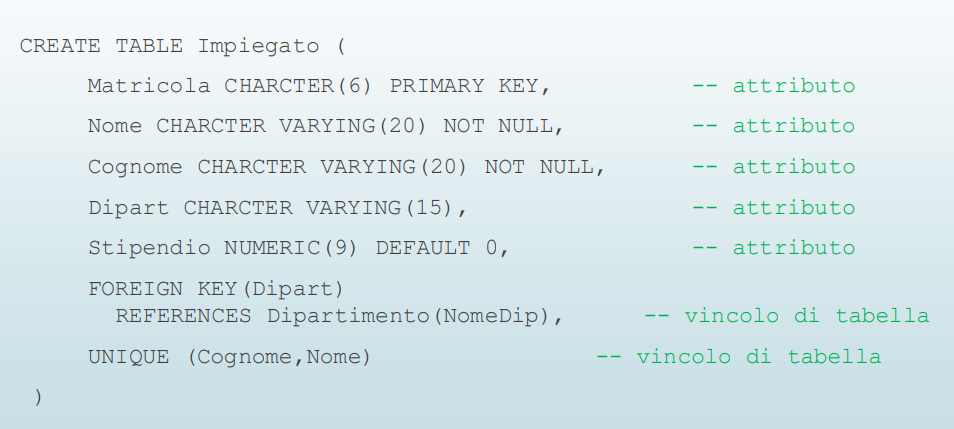
\includegraphics[width=1\linewidth]{image183}
	\caption{Esempio creazione tabella}
	\label{fig:image183}
\end{figure}
\subsubsection{Concetti fondamentali del DDL}
Già con l'istruzione \texttt{CREATE TABLE} è necessario conoscere alcuni concetti fondamentali del \textbf{Data Definition Language (DDL)}:

\begin{itemize}
	
	\item \textbf{Identificatori}
	\item \textbf{Domini} (tipi di dato)
	\item \textbf{Vincoli}
	
\end{itemize}
\subsubsection*{Gli Identificatori}
Gli \textbf{identificatori SQL} sono stringhe utilizzate per assegnare un nome agli elementi del database, come tabelle, attributi, vincoli, ecc.

\begin{itemize}
	
	\item Un identificatore deve iniziare con una \textbf{lettera (UTF-8)} oppure con un \textbf{underscore (\_)}.
	
	\item Può contenere anche \textbf{cifre} (\texttt{0--9}) e altri caratteri validi.
	
	\item Gli identificatori SQL \textbf{non sono sensibili alle maiuscole e minuscole}.
	
\end{itemize}

Ad esempio:

\begin{verbatim}
	idPersona
	idpersona
\end{verbatim}

rappresentano lo \textbf{stesso identificatore}.

Tutti i nomi utilizzati nel database, come \textbf{nomi di tabelle, attributi, indici o vincoli}, sono identificatori SQL.
\subsubsection*{Domini}
Un \textbf{dominio} definisce il \textbf{tipo di valori} che un attributo può assumere all'interno di una relazione.

SQL mette a disposizione diversi \textbf{domini elementari predefiniti}, ma consente anche di definire \textbf{domini personalizzati}.

\subsubsection*{Caratteri}

Permettono di rappresentare \textbf{singoli caratteri oppure stringhe}.

Un carattere o una stringa di caratteri viene rappresentato tra apici:

\begin{verbatim}
	'a'
	'Questa è una stringa'
\end{verbatim}

La lunghezza delle stringhe può essere \textbf{fissa} o \textbf{variabile}:

\begin{verbatim}
	CHARACTER [VARYING][(lunghezza)]
\end{verbatim}

\begin{itemize}
	
	\item \textbf{CHARACTER}: rappresenta un carattere singolo.
	
	\item \textbf{CHARACTER(20)}: stringa di lunghezza fissa.  
	Se si assegna una stringa di lunghezza inferiore a 20, la stringa viene riempita con spazi fino a raggiungere la lunghezza specificata.
	
	\item \textbf{CHARACTER VARYING(20)}: stringa di lunghezza variabile con lunghezza massima pari a 20.
	
	\item \textbf{TEXT}: stringa di lunghezza variabile senza limite prefissato.  
	Questo tipo è una \textbf{estensione specifica di PostgreSQL}.
	
\end{itemize}

\subsubsection*{Boolean}

Permettono di rappresentare \textbf{valori logici}:

\begin{verbatim}
	BOOLEAN
\end{verbatim}

I valori possibili sono:

\begin{itemize}
	
	\item \textbf{TRUE}
	\item \textbf{FALSE}
	\item \textbf{NULL} (valore sconosciuto)
	
\end{itemize}

Possono essere rappresentati anche con forme equivalenti come:

\begin{verbatim}
	TRUE / FALSE
	t / f
	1 / 0
	yes / no
\end{verbatim}

\subsubsection*{Numerici esatti}

Permettono di rappresentare \textbf{valori numerici esatti}, interi oppure con parte decimale di lunghezza prefissata.

\paragraph{Valori interi}

\begin{itemize}
	
	\item \textbf{SMALLINT}  
	Valori interi su 2 byte: da $-32768$ a $+32767$.
	
	\item \textbf{INTEGER}  
	Valori interi su 4 byte: da $-2147483648$ a $+2147483647$.
	
\end{itemize}

\paragraph{Valori decimali}

\begin{itemize}
	
	\item \textbf{NUMERIC [(precisione [, scala])]}  
	\begin{itemize}
		\item precisione: numero totale di cifre significative;
		\item scala: numero di cifre dopo la virgola.
	\end{itemize}
	
	\item \textbf{DECIMAL [(precisione [, scala])]}  
	Equivalente a \texttt{NUMERIC}.
\end{itemize}

Esempio:

\begin{verbatim}
	NUMERIC(5,2)
\end{verbatim}

Permette valori come:

\begin{verbatim}
	100.01
	100.999 -> arrotondato a 101.00
\end{verbatim}

ma non valori come:

\begin{verbatim}
	1000.01
\end{verbatim}

\subsubsection*{Numerici approssimati}

Permettono di rappresentare numeri in \textbf{virgola mobile}.

\begin{itemize}
	
	\item \textbf{REAL}: precisione di circa 6 cifre decimali.
	
	\item \textbf{DOUBLE PRECISION}: precisione di circa 15 cifre decimali.
	
\end{itemize}

Ogni numero è rappresentato tramite:

\begin{itemize}
	
	\item \textbf{mantissa} (numero frazionario)
	\item \textbf{esponente} (numero intero)
	
\end{itemize}

Il valore si ottiene moltiplicando la mantissa per $10^{esponente}$.

Esempi:

\begin{verbatim}
	0.17E16 = 1.7 x 10^15
	-0.4E-6 = -4 x 10^-7
\end{verbatim}

\textbf{Nota importante}

\begin{itemize}
	
	\item \texttt{REAL} e \texttt{DOUBLE PRECISION} sono valori \textbf{approssimati}.
	\item Se si devono rappresentare \textbf{importi di denaro}, non bisogna usare questi tipi, ma utilizzare:
	
	\begin{verbatim}
		NUMERIC(precisione)
	\end{verbatim}
	
\end{itemize}

\subsubsection*{Istanti temporali}

Permettono di rappresentare \textbf{momenti specifici nel tempo}.

\begin{itemize}
	
	\item \textbf{DATE}
	
	Rappresenta istanti nel formato:
	
	\begin{verbatim}
		YYYY-MM-DD
	\end{verbatim}
	
	Esempio:
	
	\begin{verbatim}
		'2025-03-10'
	\end{verbatim}
	
	\item \textbf{TIME [(precisione)] [WITH TIME ZONE]}
	
	Rappresenta istanti del tipo:
	
	\begin{verbatim}
		hour : minute : second
	\end{verbatim}
	
	\begin{itemize}
		\item \textbf{precisione}: numero di cifre decimali per le frazioni di secondo
		\item \textbf{WITH TIME ZONE}: permette di specificare il fuso orario
	\end{itemize}
	
	\item \textbf{TIMESTAMP [(precisione)] [WITH TIME ZONE]}
	
	Rappresenta una combinazione di:
	
	\begin{itemize}
		\item data
		\item ora
	\end{itemize}
	
\end{itemize}

\subsubsection*{Intervalli temporali}

Permettono di rappresentare \textbf{durate o intervalli di tempo}.

Sintassi generale:

\begin{verbatim}
	INTERVAL PrimaUnitàDiTempo [TO UltimaUnitàDiTempo]
\end{verbatim}

Le unità temporali sono divise in due gruppi:

\begin{itemize}
	
	\item \textbf{YEAR - MONTH}
	
	\item \textbf{DAY - HOUR - MINUTE - SECOND}
	
\end{itemize}

Esempi:

\begin{verbatim}
	INTERVAL YEAR
	INTERVAL MONTH
	INTERVAL YEAR TO MONTH
	INTERVAL DAY
	INTERVAL DAY TO HOUR
	INTERVAL DAY TO MINUTE
	INTERVAL DAY TO SECOND
\end{verbatim}

\subsubsection*{Domini definiti dall'utente}

SQL consente di definire \textbf{nuovi domini personalizzati} basati su domini esistenti.

Sintassi:

\begin{verbatim}
	CREATE DOMAIN nome AS tipoBase [valoreDefault] [vincolo]
\end{verbatim}

Il dominio definito può essere utilizzato nelle definizioni delle relazioni e può includere:

\begin{itemize}
	\item valori di default
	\item vincoli
\end{itemize}

Esempio:

\begin{verbatim}
	CREATE DOMAIN giorniSettimana AS CHARACTER(3)
	CHECK (VALUE IN ('LUN','MAR','MER','GIO','VEN','SAB','DOM'));
\end{verbatim}

In questo esempio viene definito un dominio che rappresenta i giorni della settimana tramite una stringa di tre caratteri.
\subsection{Vincoli intrarelazionali}

I \textbf{vincoli intrarelazionali} sono vincoli che si applicano agli attributi
di una singola relazione e permettono di garantire la correttezza dei dati.

I principali vincoli sono:

\begin{itemize}
	\item \textbf{NOT NULL}
	\item \textbf{UNIQUE}
	\item \textbf{PRIMARY KEY}
	\item \textbf{CHECK}
\end{itemize}

\subsubsection*{NOT NULL e DEFAULT}

Il vincolo \textbf{NOT NULL} impone che il valore dell’attributo non possa essere nullo.

Questo significa che il valore deve sempre essere specificato, oppure deve essere
presente un valore di default.

Il vincolo \textbf{DEFAULT} permette di specificare un valore predefinito quando
il comando di inserimento non fornisce alcun valore per quell’attributo.

Esempio:

\begin{verbatim}
	nome VARCHAR(20) NOT NULL
	cognome VARCHAR(20) NOT NULL DEFAULT 'VUOTO'
\end{verbatim}

\subsubsection*{UNIQUE}

Il vincolo \textbf{UNIQUE} impone che i valori di un attributo (o di un insieme di
attributi) costituiscano una \textbf{superchiave}.  
Di conseguenza, due tuple della tabella non possono avere gli stessi valori
per quegli attributi.

Può essere definito su:

\begin{itemize}
	\item un singolo attributo;
	\item un insieme di attributi.
\end{itemize}

Esempio con vincolo su più attributi:

\begin{verbatim}
	Nome VARCHAR(20),
	Cognome VARCHAR(20),
	UNIQUE(Nome, Cognome)
\end{verbatim}

In questo caso non possono esistere due righe con lo stesso
\texttt{Nome} e \texttt{Cognome} contemporaneamente.

Esempio con vincoli separati:

\begin{verbatim}
	Nome VARCHAR(20) UNIQUE,
	Cognome VARCHAR(20) UNIQUE
\end{verbatim}

In questo caso non possono esistere due righe con lo stesso
\texttt{Nome} oppure con lo stesso \texttt{Cognome}.

\subsubsection*{PRIMARY KEY}

Il vincolo \textbf{PRIMARY KEY} identifica l'attributo (o l'insieme di attributi)
che rappresenta la \textbf{chiave primaria} della relazione.

Caratteristiche:

\begin{itemize}
	\item può essere definito una sola volta per tabella;
	\item implica automaticamente il vincolo \textbf{NOT NULL}.
\end{itemize}

Esistono due modalità di definizione.

\textbf{1. Nella definizione dell'attributo} (chiave primaria singola):

\begin{verbatim}
	matricola CHAR(6) PRIMARY KEY
\end{verbatim}

\textbf{2. Come vincolo di tabella} (chiave primaria composta):

\begin{verbatim}
	nome VARCHAR(20),
	cognome VARCHAR(20),
	PRIMARY KEY(nome, cognome)
\end{verbatim}

\subsubsection*{CHECK}

Il vincolo \textbf{CHECK} permette di specificare una condizione che
deve essere soddisfatta dai valori della tabella.

Un vincolo CHECK è soddisfatto se la sua espressione è:

\begin{itemize}
	\item \textbf{vera}
	\item oppure \textbf{NULL}
\end{itemize}

Esempio:

\begin{verbatim}
	CREATE TABLE Impiegato (
	matricola CHAR(6) PRIMARY KEY,
	nome VARCHAR(20) NOT NULL,
	cognome VARCHAR(20) NOT NULL,
	qualifica VARCHAR(20),
	stipendio NUMERIC(8,2) DEFAULT 500.00 NOT NULL
	CHECK (stipendio >= 0.0), -- check di attributo
	UNIQUE(cognome, nome),
	CHECK (nome <> cognome) -- check di tabella
	);
\end{verbatim}

In questo esempio:

\begin{itemize}
	\item \texttt{CHECK(stipendio >= 0.0)} è un \textbf{check di attributo};
	\item \texttt{CHECK(nome <> cognome)} è un \textbf{check di tabella}.
\end{itemize}
\subsection{Vincoli interrelazionali}

Un \textbf{vincolo di integrità referenziale} (o \textbf{vincolo interrelazionale})
crea un legame tra i valori di un attributo (o di un insieme di attributi)
di una tabella e i valori di un attributo (o di un insieme di attributi)
di un'altra tabella.

In particolare:

\begin{itemize}
	
	\item Il vincolo collega un attributo (o insieme di attributi) $A$ della
	\textbf{tabella corrente} (detta \textbf{interna} o \textbf{slave})
	
	\item con un attributo (o insieme di attributi) $B$ di un'altra tabella
	(detta \textbf{esterna} o \textbf{master})
	
\end{itemize}

Il vincolo impone che:

\begin{itemize}
	
	\item per ogni tupla della tabella interna, il valore di $A$, se diverso da
	\texttt{NULL}, deve essere presente tra i valori di $B$ nella tabella esterna;
	
	\item l'attributo $B$ della tabella esterna deve essere soggetto a un vincolo
	\textbf{UNIQUE} oppure \textbf{PRIMARY KEY};
	
	\item l'attributo (o insieme di attributi) $B$ non deve necessariamente essere
	la chiave primaria, ma deve comunque identificare in modo univoco le tuple
	della tabella esterna.
	
\end{itemize}

\subsubsection*{FOREIGN KEY e REFERENCES}

I costrutti \textbf{REFERENCES} e \textbf{FOREIGN KEY} permettono di definire
vincoli di integrità referenziale.

Esistono due modalità di definizione.

\subsubsection*{Vincolo su un singolo attributo}

Se il vincolo coinvolge un solo attributo, è possibile utilizzare direttamente
\texttt{REFERENCES} nella dichiarazione dell'attributo, specificando la tabella
esterna e l'attributo corrispondente.

Esempio:

\begin{verbatim}
	CREATE TABLE Impiegato (
	matricola CHAR(6) PRIMARY KEY,
	reparto INTEGER REFERENCES Reparto(idReparto)
	);
\end{verbatim}

In questo caso l'attributo \texttt{reparto} della tabella \texttt{Impiegato}
fa riferimento all'attributo \texttt{idReparto} della tabella \texttt{Reparto}.

\subsubsection*{Vincolo su più attributi}

Quando il vincolo coinvolge più attributi, oppure si preferisce dichiararlo
separatamente, si utilizza il costrutto \textbf{FOREIGN KEY} alla fine della
definizione degli attributi.

Si elencano gli attributi della tabella interna e si specificano gli
attributi corrispondenti della tabella esterna tramite \texttt{REFERENCES}.

Esempio:

\begin{verbatim}
	CREATE TABLE Iscrizione (
	matricola CHAR(6),
	codiceCorso CHAR(5),
	FOREIGN KEY (matricola)
	REFERENCES Studente(matricola)
	);
\end{verbatim}

In questo modo si definisce un vincolo di integrità referenziale tra
le due tabelle.
\begin{figure}[H]
	\centering
	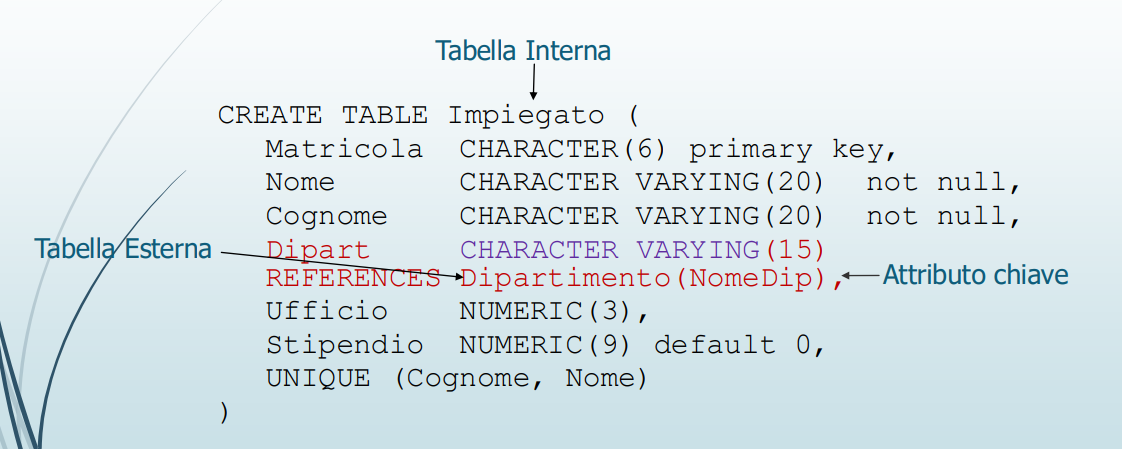
\includegraphics[width=1\linewidth]{image184}
	\caption{References e Foreign key}
	\label{fig:image184}
\end{figure}
\begin{figure}[H]
	\centering
	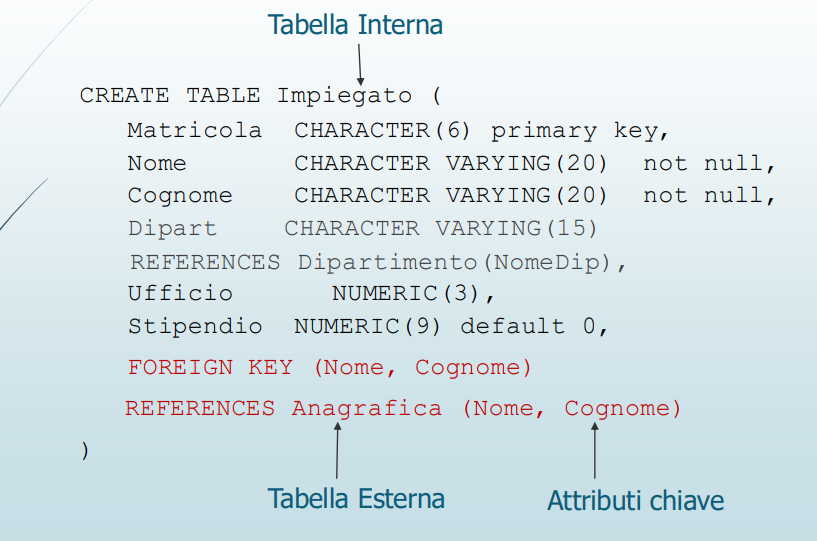
\includegraphics[width=1\linewidth]{image185}
	\caption{}
	\label{fig:image185}
\end{figure}
\begin{figure}[H]
	\centering
	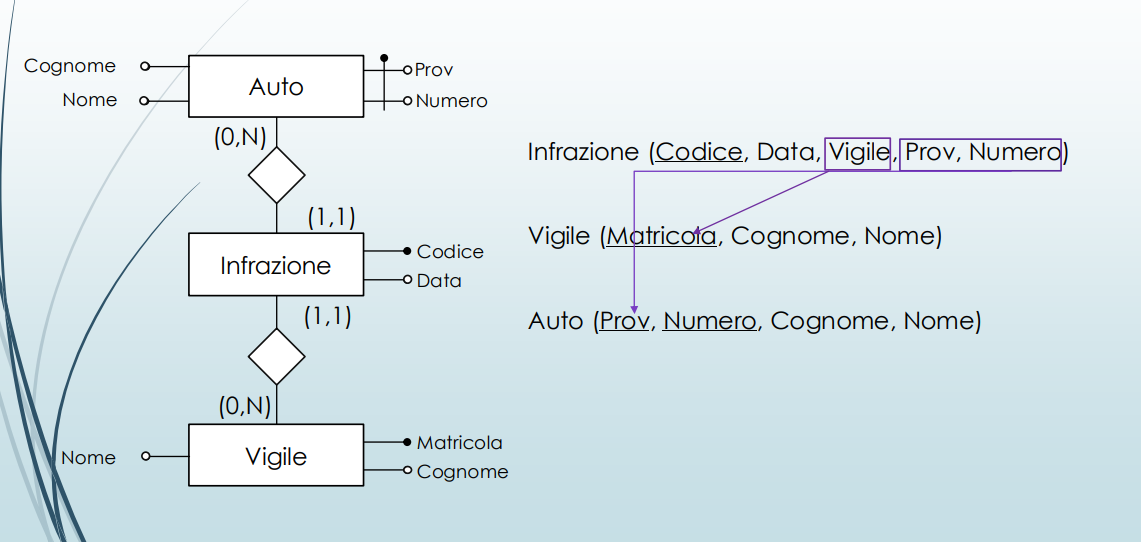
\includegraphics[width=1\linewidth]{image186}
	\caption{Esempio}
	\label{fig:image186}
\end{figure}
\begin{figure}[H]
	\centering
	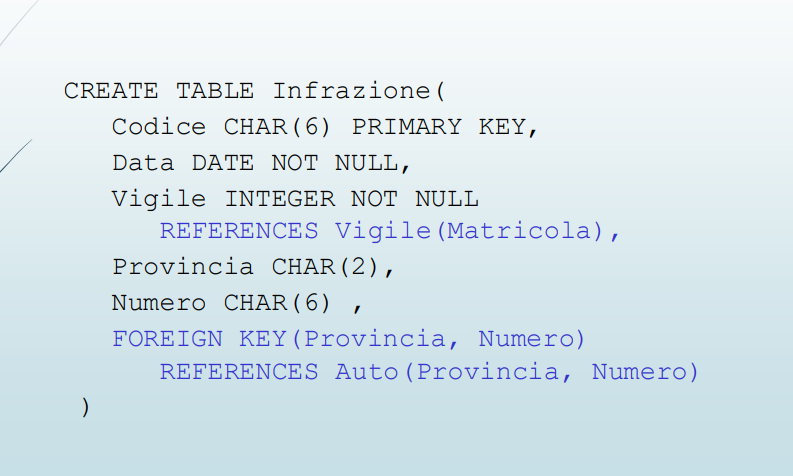
\includegraphics[width=1\linewidth]{image187}
	\caption{Risoluzione Esempio}
	\label{fig:image187}
\end{figure}
\subsection{Modifica ed eliminazione delle strutture}

SQL mette a disposizione diversi comandi per modificare o eliminare
gli elementi di una base di dati, come domini, tabelle e attributi.

\begin{itemize}
	
	\item \textbf{ALTER}: permette di effettuare modifiche alla struttura
	di domini e tabelle (ad esempio aggiungere o modificare colonne).
	
	\item \textbf{DROP DOMAIN}: permette di rimuovere un dominio.
	
	\item \textbf{DROP TABLE}: permette di eliminare una tabella dal database.
	
\end{itemize}

\subsubsection*{Aggiunta di un attributo}

Un nuovo attributo può essere aggiunto a una tabella tramite il comando
\texttt{ADD COLUMN}.

Sintassi generale:

\begin{verbatim}
	ALTER TABLE tabella ADD COLUMN attributo tipo;
\end{verbatim}

Esempio:

\begin{verbatim}
	ALTER TABLE impiegato ADD COLUMN stipendio NUMERIC(8,2);
\end{verbatim}

\subsubsection*{Rimozione di un attributo}

Un attributo può essere rimosso da una tabella tramite il comando
\texttt{DROP COLUMN}.

Sintassi generale:

\begin{verbatim}
	ALTER TABLE tabella DROP COLUMN attributo;
\end{verbatim}

Esempio:

\begin{verbatim}
	ALTER TABLE impiegato DROP COLUMN stipendio;
\end{verbatim}

\subsubsection*{Modifica del valore di default}

È possibile modificare o rimuovere il valore di default di un attributo
tramite il comando \texttt{ALTER COLUMN}.

Sintassi:

\begin{verbatim}
	ALTER TABLE tabella 
	ALTER COLUMN attributo {SET DEFAULT valore | DROP DEFAULT};
\end{verbatim}

Esempio:

\begin{verbatim}
	ALTER TABLE impiegato 
	ALTER COLUMN stipendio SET DEFAULT 1000.00;
\end{verbatim}

\subsection{Cancellazione dei dati}

Le tuple di una tabella possono essere eliminate tramite il comando
\texttt{DELETE}.

Sintassi generale:

\begin{verbatim}
	DELETE FROM tabella [WHERE condizione];
\end{verbatim}

\begin{itemize}
	
	\item \texttt{condizione} è un'espressione booleana che seleziona
	le tuple da cancellare.
	
	\item Se la clausola \texttt{WHERE} non è presente,
	\textbf{tutte le tuple della tabella vengono cancellate}.
	
\end{itemize}

Esempio:

\begin{verbatim}
	DELETE FROM impiegato WHERE matricola = 'A001';
\end{verbatim}

\subsubsection{Eliminazione di una tabella}

Una tabella può essere eliminata completamente dal database tramite
il comando \texttt{DROP TABLE}.

Sintassi:

\begin{verbatim}
	DROP TABLE tabella;
\end{verbatim}